\section{Problem 3}

{\bfseries 3.1 Part 1}

We have conducted a series of experimentation with the simple data from Bishop's Figure 1.4

%TODO: generate graphs to show the impact of increasing M (overfitting), but this is shown in the previou squestion
As M increases, the curve is more likely to overfit the data. 

We have conducted a series of experiments using M =1, M = 3 and M = 9 with varying lambdas. 


\begin{figure}[!htb]
\minipage{0.32\textwidth}
  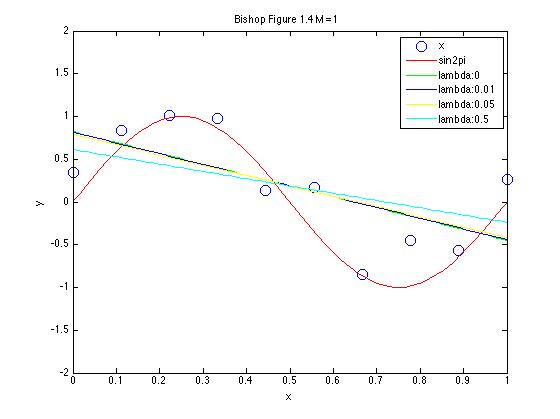
\includegraphics[width=\linewidth]{figures/p3_bishop_m=1}
  \caption{M = 1}\label{fig:figures/p3_bishop_m=1}
\endminipage\hfill
\minipage{0.32\textwidth}
  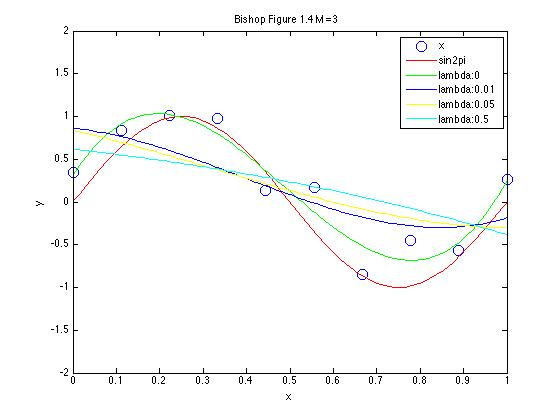
\includegraphics[width=\linewidth]{figures/p3_bishop_m=3}
  \caption{M = 3}\label{fig:figures/p3_bishop_m=3}
\endminipage\hfill
\minipage{0.32\textwidth}%
  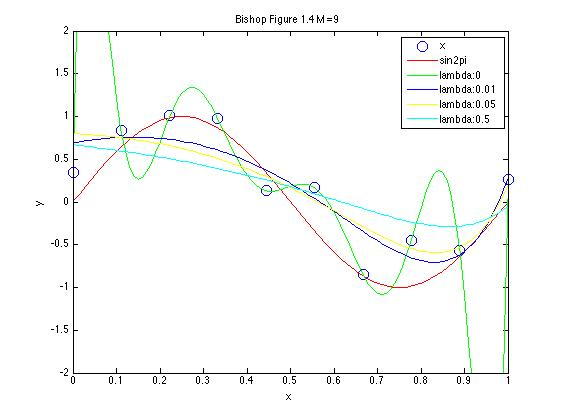
\includegraphics[width=\linewidth]{figures/p3_bishop_m=9}
  \caption{M = 9}\label{fig:figures/p3_bishop_m=9}
\endminipage\hfill

\end{figure}



\begin{figure}{h}
\end{figure}


%% \begin{figure}[h]

%%   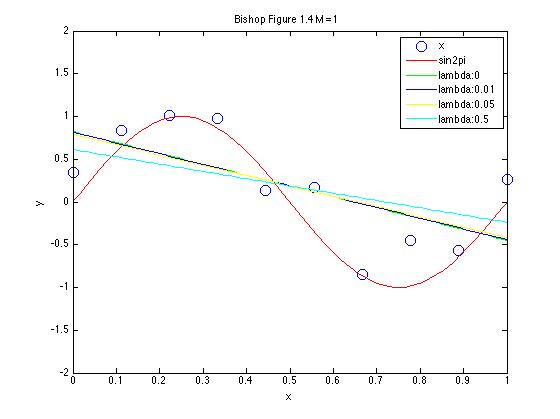
\includegraphics[width=0.5\textwidth]{figures/p3_bishop_m=1}
%%   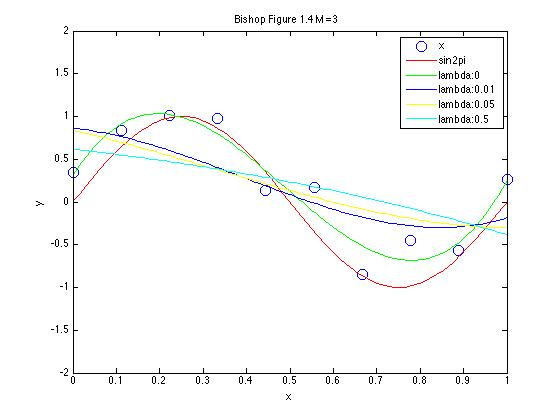
\includegraphics[width=0.5\textwidth]{figures/p3_bishop_m=3}
%%   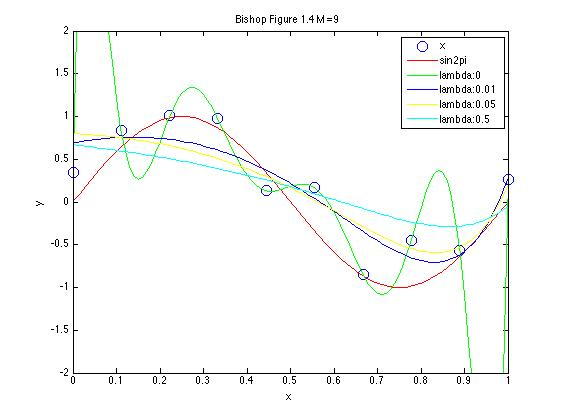
\includegraphics[width=0.5\textwidth]{figures/p3_bishop_m=9}

%% \end{figure}

we can see that for a smaller M, changing the lambda doesn't impact the performance as much. It bends the graph in the more general direction. For a large M, the lambda greatly reduces the overfitting problem. As a result, even with a large M, the model can be more generalized. 

{\bfseries 3.2 Part 2}

First, we can see that in general error from training set B is higher than that from training set A. 
This is because there is a outlier in trainng set B. This prevented us from creating a good model. 


\begin{figure}[!htb]
\minipage{0.32\textwidth}
  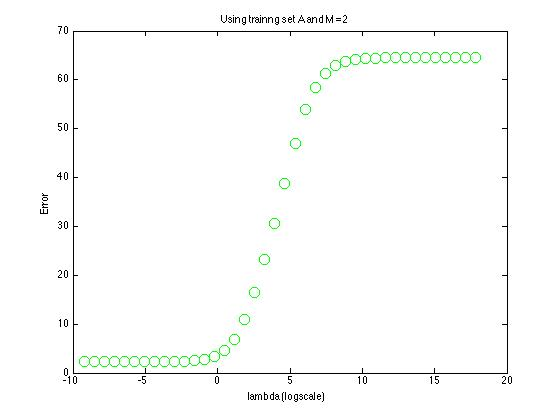
\includegraphics[width=\linewidth]{figures/p3_regressA_m=2}
  \caption{M = 2}\label{fig:figures/p3_regressA_m=2}
\endminipage\hfill
\minipage{0.32\textwidth}
  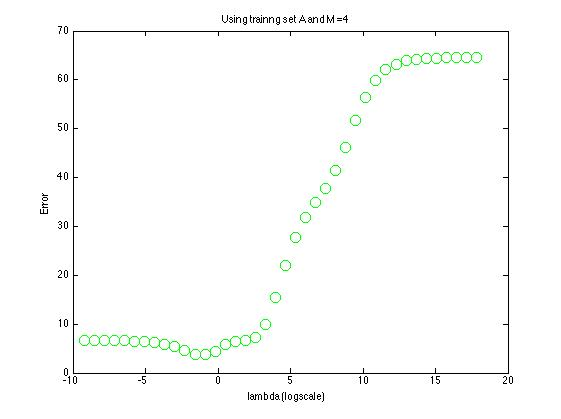
\includegraphics[width=\linewidth]{figures/p3_regressA_m=4}
  \caption{M = 4}\label{fig:figures/p3_regressA_m=4}
\endminipage\hfill
\minipage{0.32\textwidth}%
  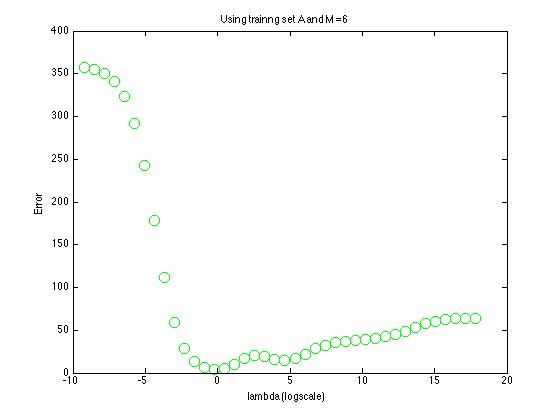
\includegraphics[width=\linewidth]{figures/p3_regressA_m=6}
  \caption{M = 6}\label{fig:figures/p3_regressA_m=6}
\endminipage
\end{figure}


\begin{figure}[!htb]
\minipage{0.32\textwidth}
  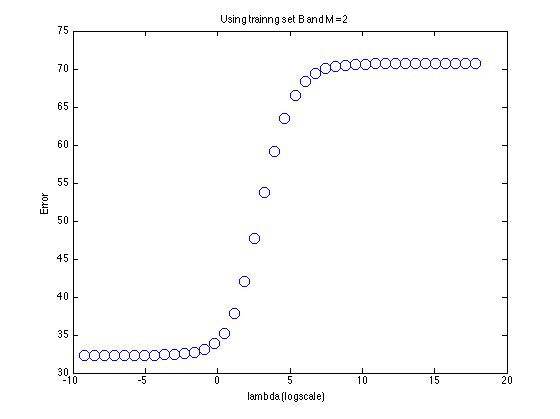
\includegraphics[width=\linewidth]{figures/p3_regressB_m=2}
  \caption{M = 2}\label{fig:figures/p3_regressB_m=2}
\endminipage\hfill
\minipage{0.32\textwidth}
  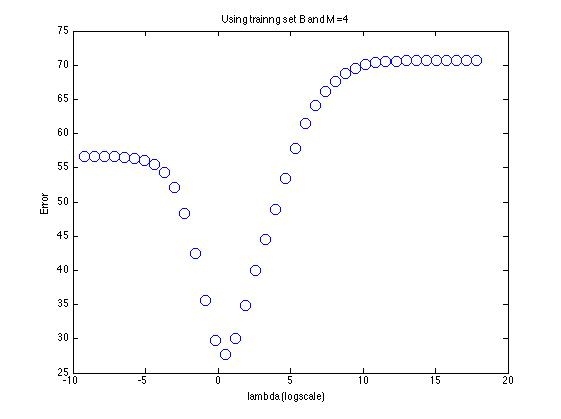
\includegraphics[width=\linewidth]{figures/p3_regressB_m=4}
  \caption{M = 4}\label{fig:figures/p3_regressB_m=4}
\endminipage\hfill
\minipage{0.32\textwidth}%
  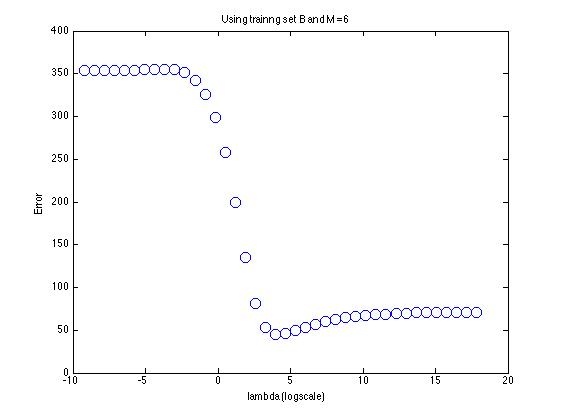
\includegraphics[width=\linewidth]{figures/p3_regressB_m=6}
  \caption{M = 6}\label{fig:figures/p3_regressB_m=6}
\endminipage
\end{figure}


The best configurtion from the model in A is with M = 2; The error is alredy very small. Increasing
the lambda actually increases the error rate quickly. 

As we incrase M, the error incrases as the model overfits the original traning A data. However, we 
can see the effect of regularing the weight. The error rate decreases as we increase the size of lambda. However, after the minimum point, the error goes up again as the weight factors are no longer guided by the training data set. 

For training data B, we can see the error with lambda = 0 is much larger compare to A. This is because there is an outlier in the traning data B. 


{\bfseries 3.3 Part3}
\begin{figure}[!htb]
  \minipage{0.48\textwidth}
  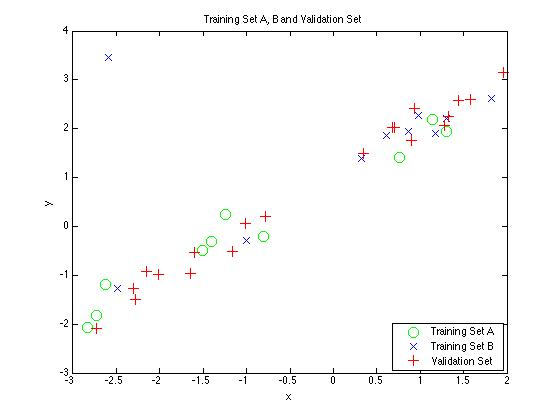
\includegraphics[width=\linewidth]{figures/p3_training_validation_data}
  \caption{Training and Validation Data}\label{fig:figures/p3_training_validation_data}
  \endminipage\hfill
  \minipage{0.48\textwidth}%
  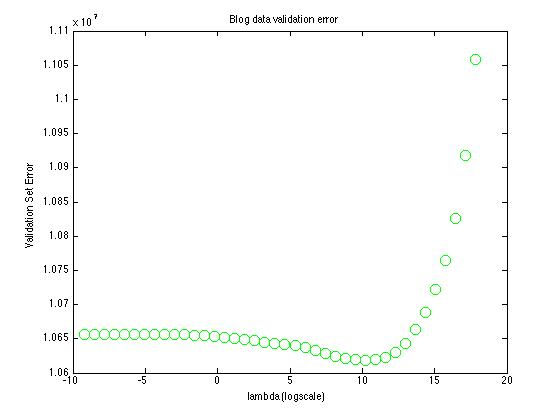
\includegraphics[width=\linewidth]{figures/p3_blogdata_lambda}
  \caption{Blog validation data error}
  \endminipage\hfill
\end{figure}

This shows that as we increase the value of lambda, the error first decreases. However, as we futher
increase lambda, the weight vectors no longer rely on the data, the error increases quickly. 


Even with the best lambda we chose from the validation set, the error for the test set is still large
in the order of $10^{7}$. However, we belive that this is because the simple linear model (without non-linear basis functions) is unable to accurately describe a model. 
